\documentclass{tufte-handout}

\title{Math 451, Homework Set \#1}
\author{Anthony Brice}

\usepackage{graphicx} % allow embedded images
\setkeys{Gin}{width=\linewidth,totalheight=\textheight,keepaspectratio}
% \graphicspath{{graphics/}} % set of paths to search for images
\usepackage{amsmath, amsthm, amssymb}  % extended mathematics
\usepackage{booktabs} % book-quality tables
\usepackage{units}    % non-stacked fractions and better unit spacing
\usepackage{multicol} % multiple column layout facilities
\usepackage{lipsum}   % filler text
\usepackage{fancyvrb} % extended verbatim environments
  \fvset{fontsize=\normalsize}% default font size for fancy-verbatim
                              % environments
% Standardize command font styles and environments
\newcommand{\doccmd}[1]{\texttt{\textbackslash#1}}% command name -- adds backslash automatically
\newcommand{\docopt}[1]{\ensuremath{\langle}\textrm{\textit{#1}}\ensuremath{\rangle}}% optional command argument
\newcommand{\docarg}[1]{\textrm{\textit{#1}}}% (required) command argument
\newcommand{\docenv}[1]{\textsf{#1}}% environment name
\newcommand{\docpkg}[1]{\texttt{#1}}% package name
\newcommand{\doccls}[1]{\texttt{#1}}% document class name
\newcommand{\docclsopt}[1]{\texttt{#1}}% document class option name
\newenvironment{docspec}{\begin{quote}\noindent}{\end{quote}}% command
                                % specification environment
\newcommand{\e}[1]{\ensuremath{\times 10^{#1}}} % Macro for scientific notation

% Use fancy symbols for footnotes
\usepackage{hyperref}
\usepackage{natbib}
\renewcommand{\thefootnote}{\fnsymbol{footnote}}
\usepackage{perpage}
\MakePerPage{footnote}

\renewcommand{\thefootnote}{\fnsymbol{footnote}}

\begin{document}

\maketitle

\section{Problem 1}
\begin{description}
<<<<<<< HEAD
  \item \textit{Convert the following complex numbers into polar form
      and exponentiated form.
      \footnote{$a - bi = r(\cos\theta + i\sin\theta) = re^{i\theta}$,
      where $r = \sqrt{a^2 + b^2}$ and $\tan\theta = a/b.$\\
      $a = r\cos\theta$. Usually $r \geq 0$ and $\theta \in (-\pi,
      \pi]$.)}}
  \item[(a)] $7 + 7i\sqrt{3}$
  \item[(b)] $-2 + 2i$
  \item[(c)] $-16$
  \item[(d)] $27i$
\end{description}

=======
\item \textit{Convert the following complex numbers into polar form
    and exponentiated form.}
\item[(a)] $7 + 7i\sqrt{3}$.
\item[(b)] $-2 + 2i$.
\item[(c)] $-16$.
\item[(d)] $27i$.
\end{description}

We will follow the same general strategy in translating each
expression. We first calculate $r$ and $\theta$ via the following
formulas. Given the complex number $a + bi$,

\begin{align*}
  r &= \sqrt{a^2 + b^2}\\
  \tan \theta &= \frac{a}{b}.
\end{align*}

Then we apply the following for polar and exponential forms, respectively.

\begin{align*}
  a + bi &= r \left( \cos \theta + i \sin \theta \right)\\
         &= r e^{i \theta}.
\end{align*}

>>>>>>> c484389cdf43de640bc2a6d9b6e1a830ab252a5f
\begin{description}
\item[\textup{(a)}]
  \begin{align*}
    7 + 7i\sqrt{3} &\Rightarrow r=\sqrt{7^2 +
                     {\left(7\sqrt{3}\right)}^2}, \, \tan\theta =
                     \sqrt{3}\\
                   &\Rightarrow r = 14\\
                   &\Rightarrow \theta = {\pi \over 3} && \footnotemark\\
    \Rightarrow 7 + 7i\sqrt{3} &= 14\left(\cos{\pi \over 3} +
                                 i\sin{\pi \over 3}\right)\\
                                 &= 14e^{i\pi / 3}.
  \end{align*}
  \footnotetext{$\tan\theta = \sqrt{3}\Rightarrow \arctan\sqrt{3} =
    \theta$.}

\item[\textup{(b)}]
  \begin{align*}
    -2 + 2i &\Rightarrow r = \sqrt{(-2)^2 + 2^2}, \, \tan \theta =
              -1\\
            &\Rightarrow r = 2 \sqrt 2\\
            &\Rightarrow \theta = {3\pi \over 4} && \footnotemark\\
    \Rightarrow -2 + 2i &= 2\sqrt2 \left(\cos{3\pi \over 4} +
                          i\sin{3\pi \over 4}\right)\\
            &= 2\sqrt2 e^{3i\pi / 4}.
  \end{align*}
  \footnotetext{$\theta \neq -\frac{\pi}{4}.$ $a < 0$ and $b > 0,$ so
    we are in the second quadrant.}

\item[\textup{(c)}]
  \begin{align*}
    -16 &\Rightarrow r = 16, \, \tan \theta = 0\\
        &\Rightarrow \theta = \pi\\
    \Rightarrow -16 &= 16(\cos \pi + i\sin \pi)\\
        &= -16\\
        &= 16e^{i\pi}.
  \end{align*}

\item[\textup{(d)}]
  \begin{align*}
    27i &= 27i \sin {\pi \over 2} && \footnotemark\\
        &= 27e^{i\pi / 2}
  \end{align*}
  \footnotetext{$\theta = \frac{\pi}{2}$ because we in the complex
    domain, baby.}
\end{description}

\section{Problem 2}
\begin{description}
\item \textit{Using the polar form, compute $(-2+2i)(7 + 7i\sqrt{3})$
    and $(7 + 7i\sqrt{3})/(-2 + 2i).$ Check your answers by computing
    these directly (without the polar or exponential forms).}
\end{description}

<<<<<<< HEAD
First we compute the polar forms.
=======
Using the polar forms computed in \textit{Problem 1}, we will apply
the following. Let
\begin{align*}
  w &= r(\cos \alpha + i \sin \alpha)\\
  z &= s(\cos \beta + i \sin \beta).
\end{align*}

Then
\begin{align*}
  wz &= rs(\cos{(\alpha + \beta)} + i \sin{(\alpha + \beta)})\\
  {w \over z} &= {r \over s} \left( \cos{ (\alpha - \beta)} + i \sin{
                (\alpha - \beta)}\right).
\end{align*}
>>>>>>> c484389cdf43de640bc2a6d9b6e1a830ab252a5f

\begin{align*}
<<<<<<< HEAD
  (-2 + 2i)\left(7 + 7i\sqrt 3\right) &= \left(2 \sqrt 2 e^{3i \pi /
                                        4}\right)\left(14e^{i\pi /
                                        3}\right). && \footnotemark \\
                                      &= 28 \sqrt 2 e^{-11i\pi / 12}.
=======
  (-2 + 2i)\left(7 + 7i\sqrt 3\right) &= 28 \sqrt 2 \left( \cos{
                                        \left( {3 \pi \over 4} + {\pi
                                        \over 3}\right)} + i \sin{
                                        \left( {3 \pi \over 4} + {\pi
                                        \over 3}\right)}\right)\\
                                      &= 28 \sqrt 2 \left( \cos{ 13
                                        \pi \over 12} + i \sin{ 13 \pi
                                        \over 12}\right).
>>>>>>> c484389cdf43de640bc2a6d9b6e1a830ab252a5f
\end{align*}
\footnotetext{\label{p2l1}Let $w = r(\cos\alpha + i\sin\alpha) = re^{i\alpha}$ and
  $z = s(\cos\beta + i\sin\beta) = se^{i\beta}.$ Then
  $wz = rs(\cos(\alpha + \beta) + i\sin(\alpha + \beta)) =
  rse^{i(\alpha + \beta)}$.}

\begin{align*}
<<<<<<< HEAD
  {7 + 7i \sqrt 3 \over -2 + 2i} &= {14e^{i\pi / 3} \over 2 \sqrt 2
                                   e^{3i\pi / 4}}. && \footnotemark \\
                                 &= 7 \sqrt 2 e^{-5 i \pi / 12}.
=======
  {7 + 7i \sqrt 3 \over -2 + 2i} &= {7 \over \sqrt 2} \left( \cos{
                                   \left( {\pi \over
                                   3} - {3 \pi \over 4} \right)} + i
                                   \sin{ \left( {\pi \over 3} - {3 \pi
                                   \over 4} \right) }\right)\\
                                 &= {7 \over \sqrt 2} \left(
                                   \cos{ \left( -{5 \pi \over 12}
                                   \right)} + i
                                   \sin{ \left( -{5 \pi \over 12}
                                   \right)} \right).\\
>>>>>>> c484389cdf43de640bc2a6d9b6e1a830ab252a5f
\end{align*}
\footnotetext{From~\ref{p2l1},
  $w / z = (r/s)(\cos(\alpha - \beta) + i\sin(\alpha -
  \beta)) = (r/s)e^{i(\alpha - \beta)}$.}

Then we compute them directly.

\begin{align*}
  (-2 + 2i)\left(7 + 7i\sqrt 3 \right) &= \left(-14 - 14 i \sqrt 3 + 14i
                                         -14 \sqrt 3\right)\\
                                       &= -14(1 + \sqrt 3) + 14i(1 -
                                         \sqrt 3)\\
                                       &= \ldots && \footnotemark
\end{align*}
\footnotetext{In this context, ``\ldots'' means I don't know what to do.}

\section{Problem 3}
\begin{description}
\item \textit{Use de Moivre's theorem to compute $(-2 + 2i)^5$ and $(7
    + 7i\sqrt 3)^4$. \footnote{De Moivre's theorem: Let $w = r(\cos\alpha + i\sin\alpha) = re^{i\alpha}.$ Then $w^n = r^n(\cos(n\alpha) + i\sin(n\alpha)) = r^n e^{in\alpha}$.}}
\end{description}

\begin{align*}
  {(-2 + 2i)}^5 &= {\left(2 \sqrt 2 e^{3 i \pi / 4} \right)}^5\\
                &= 12 \sqrt 2 e^{-i \pi / 4}. && \footnotemark
\end{align*}
\footnotetext{Add or subtract multiples of $2\pi$ from radians when
  they move outside the range.}

\begin{align*}
  {\left( 7 + 7 i \sqrt 3 \right)}^4 &= {\left( 14 e^{i \pi / 3}
                                       \right)}^4\\
                                     &= 38416 e^{-2 i \pi / 3}.
\end{align*}

\section{Problem 4}

\begin{description}
\item \textit{Find all cube roots of $27i$, and all fourth roots of
    $-16$.}
\end{description}

\begin{align*}
  \sqrt[3]{27 i} &= \sqrt[3]{27 e^{i (\pi / 2 + 2 \pi k)}} \; \forall
  \; k \in \{0,1,2\} && \footnotemark\\
                 &= 3 e^{i (\pi / 6 + 2 \pi k / 3)} \; \forall \; k
                   \in \{0,1,2\}.
\end{align*}
\footnotetext{We're looking for cube roots, therefore we must have
  $3$ of them.}

\begin{align*}
  \sqrt[4]{-16} &= \sqrt[4]{16e^{i(\pi + 2\pi k)}} \; \forall \; k \in \{0,1,2,3\}\\
                &= 2e^{i(\pi / 4 + \pi k / 2)} \; \forall \; k \in \{0,1,2,3\}.
\end{align*}

\section{Problem 5}

\begin{description}
\item \textit{Use the quadratic formula to solve
    $x^2 - (5 - i)x + (8 - 1) = 0$.}
\end{description}

\begin{align*}
  x &= {5 - i \pm \sqrt{(5 - i)^2 + 4(8 - i)} \over 2}\\
    &= {5 \over 2} - {i \over 2} \pm {1 \over 2} - {3 i \over 2}.
\end{align*}

Then $x = 3 - 2 i$ and $x = 2 + i$.

\section{Problem 6}

\begin{description}
\item \textit{Compute the eighth roots of unity. Plot them on a graph and
  connect these points. What shape do you obtain?}
\end{description}

\begin{align*}
<<<<<<< HEAD
  \sqrt[8]{1} &= \sqrt[8]{e^{2 \pi k i}} \; \forall \; k \in
                \{0,\ldots,7\}.\\
              &= e^{\pi k i / 4} \; \forall \; k \in \{0,\ldots,7\}.
\end{align*}

\begin{marginfigure}
=======
  \sqrt[8]{1} &= \sqrt[8]{e^{2 i \pi k}} \; \forall \; k \in
                \{0,\ldots,7\}\\
              &= e^{i \pi k/ 4} \; \forall \; k \in \{0,\ldots,7\}.
\end{align*}

\begin{figure}[h]
  \label{p6f1}
>>>>>>> c484389cdf43de640bc2a6d9b6e1a830ab252a5f
  \centering
  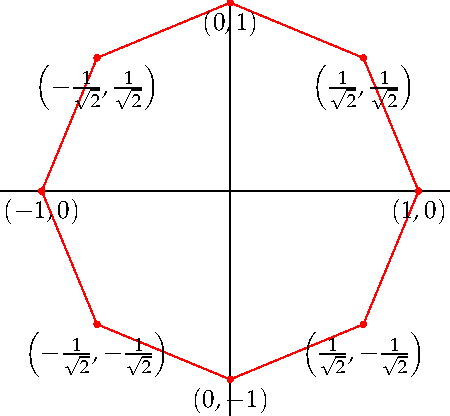
\includegraphics[height=5cm]{tpr6.pdf}
  % \input{p6.tex}
  \caption{Note that all roots lie on the unit circle.}
\end{marginfigure}

We obtain an octagon.

\section{Problem 7}

\begin{description}
\item \textit{By using Euler's Identity, show that the conjugate of
    $e^{i \theta}$ equals $e^{-i \theta}$.}\footnote{Euler's identity:
    $e^{i\theta} = \cos\theta + i\sin\theta$. That definition is often
    the first question on midterms given by Dr.\ Sittinger.}
\end{description}

\begin{align*}
  \overline{e^{i \theta}} &= \overline{\cos \theta + i \sin \theta}\\
                          &= \cos \theta - i \sin \theta && \footnotemark\\
                          &= \cos{(-\theta)} + i \sin{(-\theta)} && \footnotemark\\
                          &= e^{-i \theta}.
\end{align*}
\footnotetext[2]{$\overline{a + b} = a - b$.}  \footnotetext{$\cos$ is an
  even function, so $\cos \theta$ = $\cos(-\theta)$. Similarly, $\sin$
  is odd, so $-\sin \theta = \sin(-\theta)$.}

\end{document}
%%% Local Variables:
%%% mode: latex
%%% TeX-master: t
%%% End:

%  LocalWords:  Sittinger
